\documentclass[xcolor=svgnames,11pt]{beamer}

\usepackage{graphicx}

\usepackage[italian, english]{babel} 
\usepackage[utf8x]{inputenc}

\usepackage{hyperref}
\usepackage{tabularx}
\usepackage{url}
\usepackage{pbox}

\usetheme{Goettingen}
\definecolor{raspi}{HTML}{bb1142}
\definecolor{green_raspi}{HTML}{75aa28}
\definecolor{myblack}{RGB}{14,14,14}

\usecolortheme[named=myblack]{structure}
\beamertemplatenavigationsymbolsempty 

\beamertemplateshadingbackground{white!15}{raspi!5}
\setbeamertemplate{sidebar canvas right}[vertical shading]%
[top=myblack!30,bottom=white!90]

\mode<presentation>{\usebackgroundtemplate{
\includegraphics[height=\paperheight]{back.png}}} 

\setbeamertemplate{blocks}[rounded][shadow=false]
\setbeamercolor{block body}{bg=green_raspi!30}
\setbeamercolor{block title}{bg=green_raspi!90}

\setbeamercovered{transparent}

\title{\textbf{Raspberry Pi \\ Il computer che hai sempre voluto avere} \\ Lezione 2}
\author{Nicola Corti - Niccol\`o Pieretti}
\institute{Gruppo Utenti Linux Pisa \\ \medskip 
\includegraphics[height=1.5cm]{gulp_logo.png}}
\logo{gulp_logo.png}
\date{29 Aprile 2015}

 
\begin{document}

\begin{frame}
	\titlepage
\end{frame}

%%%%%%%%%%%%%%%%%%%%%%
\section{NOOBS}
\begin{frame}{}
\begin{center}
\begin{Huge}
{\color{green_raspi} \textbf{NOOBS}}
\end{Huge}
\end{center}
\end{frame}

\begin{frame}{Prima installazione}
\begin{block}{NOOBS}

Per la prima installazione consiglio di usare \textbf{NOOBS} (New Out Of the Box Software), un manager che ci aiuta durante l'installazione del nostro sistema operativo.

\end{block}

\pause
\medskip

NOOBS \`e sviluppato direttamente dalla Raspberry Pi Foundation, e sono presenti numerose guide che ci guideranno passo passo nella configurazione.

\pause
\medskip
\begin{center}
\url{http://www.raspberrypi.org/help/noobs-setup/}
\end{center}

\pause
\medskip

Si possono anche acquistare schede SD con NOOBS \textbf{precaricato} all'interno.

\end{frame}

\begin{frame}{1) Scaricare NOOBS}
Scaricare NOOBS dal sito internet
\begin{center}
\url{http://www.raspberrypi.org/downloads/}

\bigskip
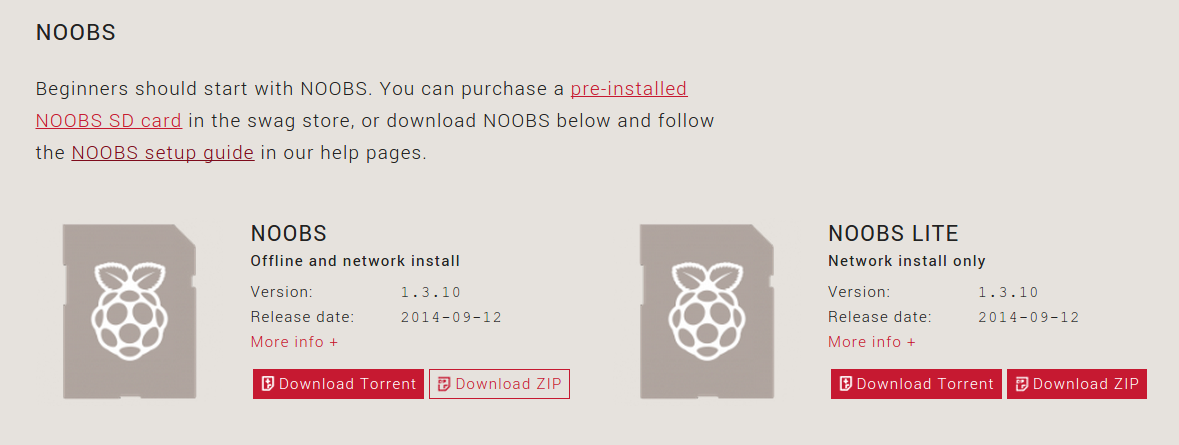
\includegraphics[width=8cm]{guide/1.png}

\end{center}
\end{frame}

\begin{frame}{2) Formattare la scheda SD}
Formattare una scheda SD da almeno \textbf{4 GB} e creare una nuova partizione con filesystem \textbf{FAT32}.

\bigskip
\begin{center}
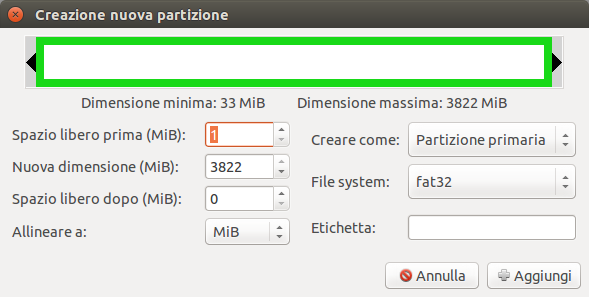
\includegraphics[width=8cm]{guide/2.png}
\end{center}
\end{frame}

\begin{frame}{3) Copiare NOOBS su scheda SD}
Copiare il contenuto dell'archivio di NOOBS dentro la scheda SD (nella root, cio\`e senza creare cartelle).

\medskip
\begin{center}
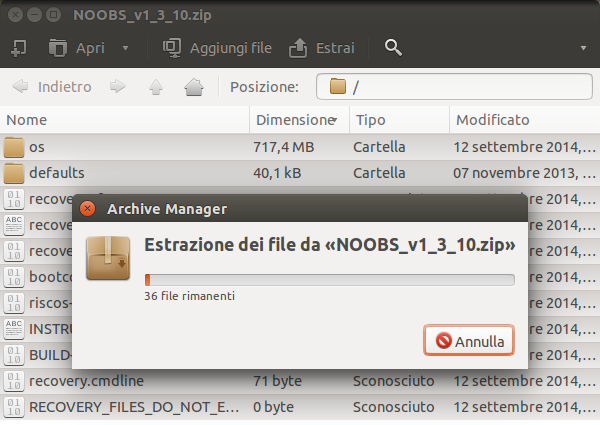
\includegraphics[width=8cm]{guide/3.png}
\end{center}
\end{frame}

\begin{frame}{4) Avviare il Raspberry Pi}
Inserire la scheda SD nel Raspberry Pi, collegare le periferiche (monitor, tastiera, etc...), collegare la rete, ed attaccare il raspberry all'alimentazione.

\medskip
\begin{center}
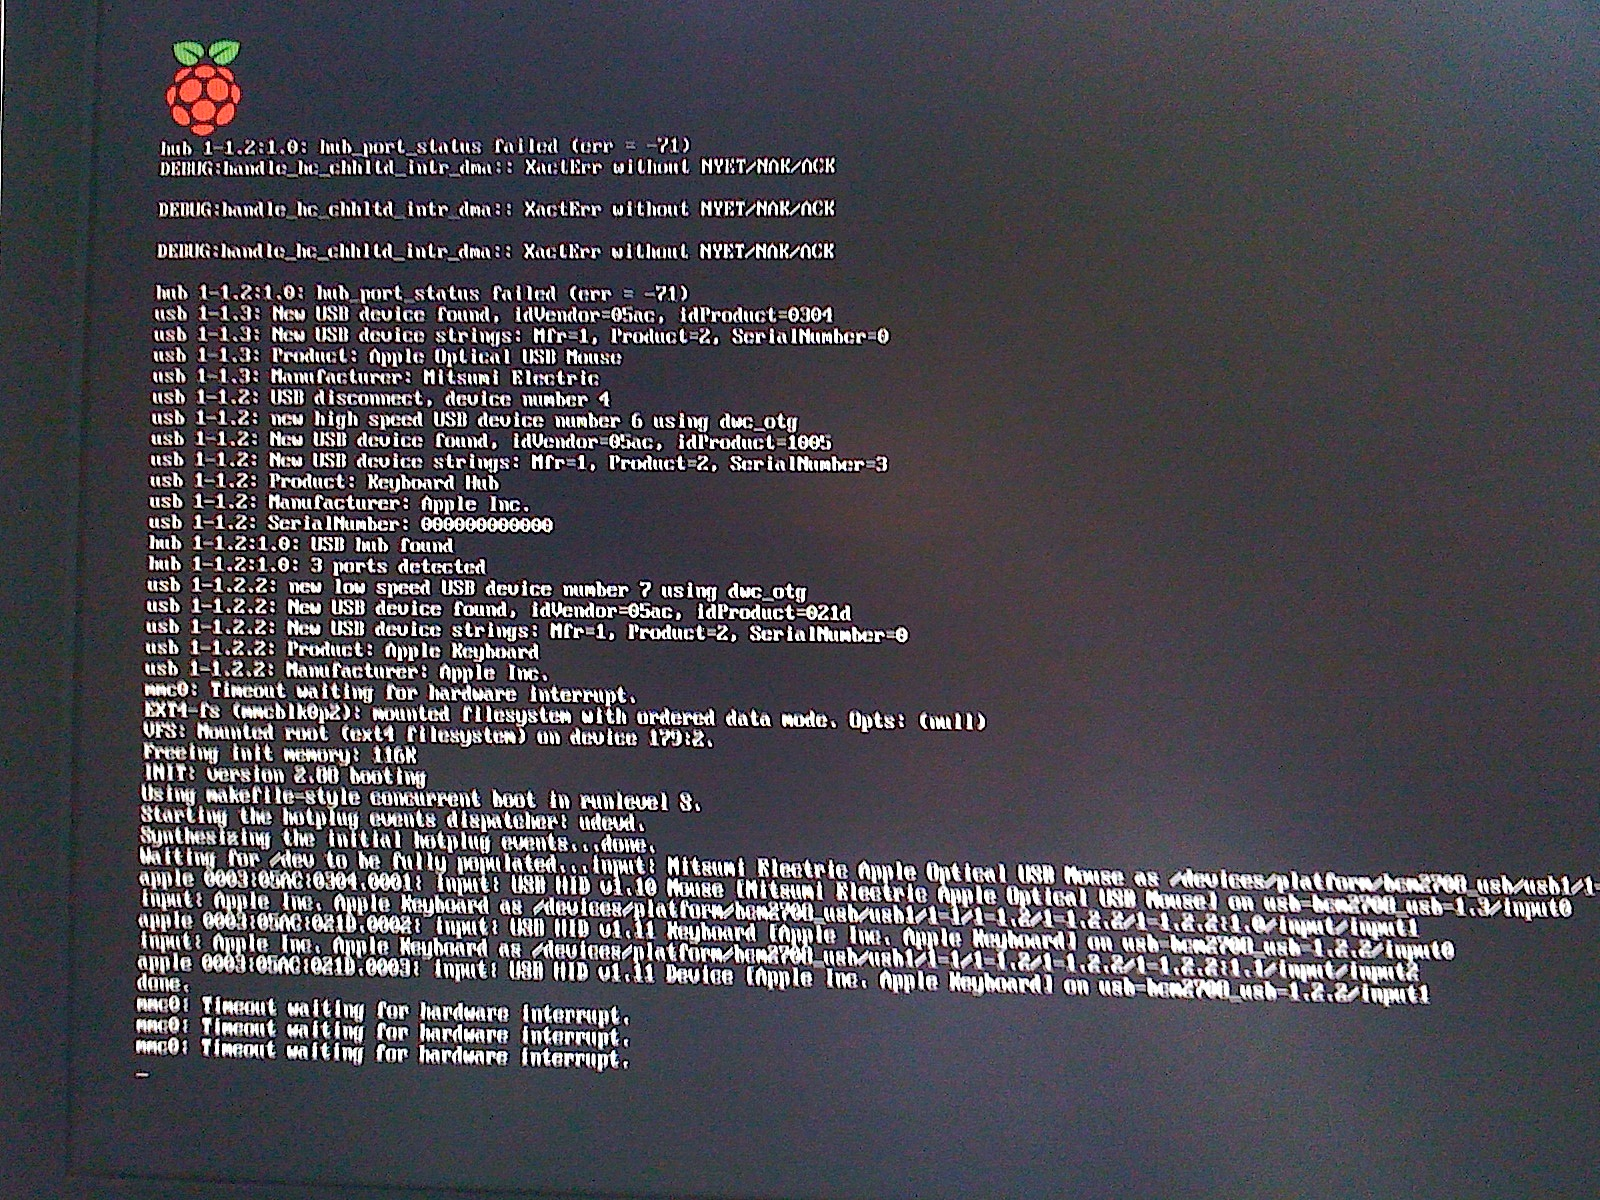
\includegraphics[width=8cm]{guide/4.jpg}
\end{center}
\end{frame}



\begin{frame}{5) Scegliere i S.O.}
Scegliere dall'elenco di Sistemi Operativi che si vogliono installare su questa scheda SD.

\medskip
\begin{center}
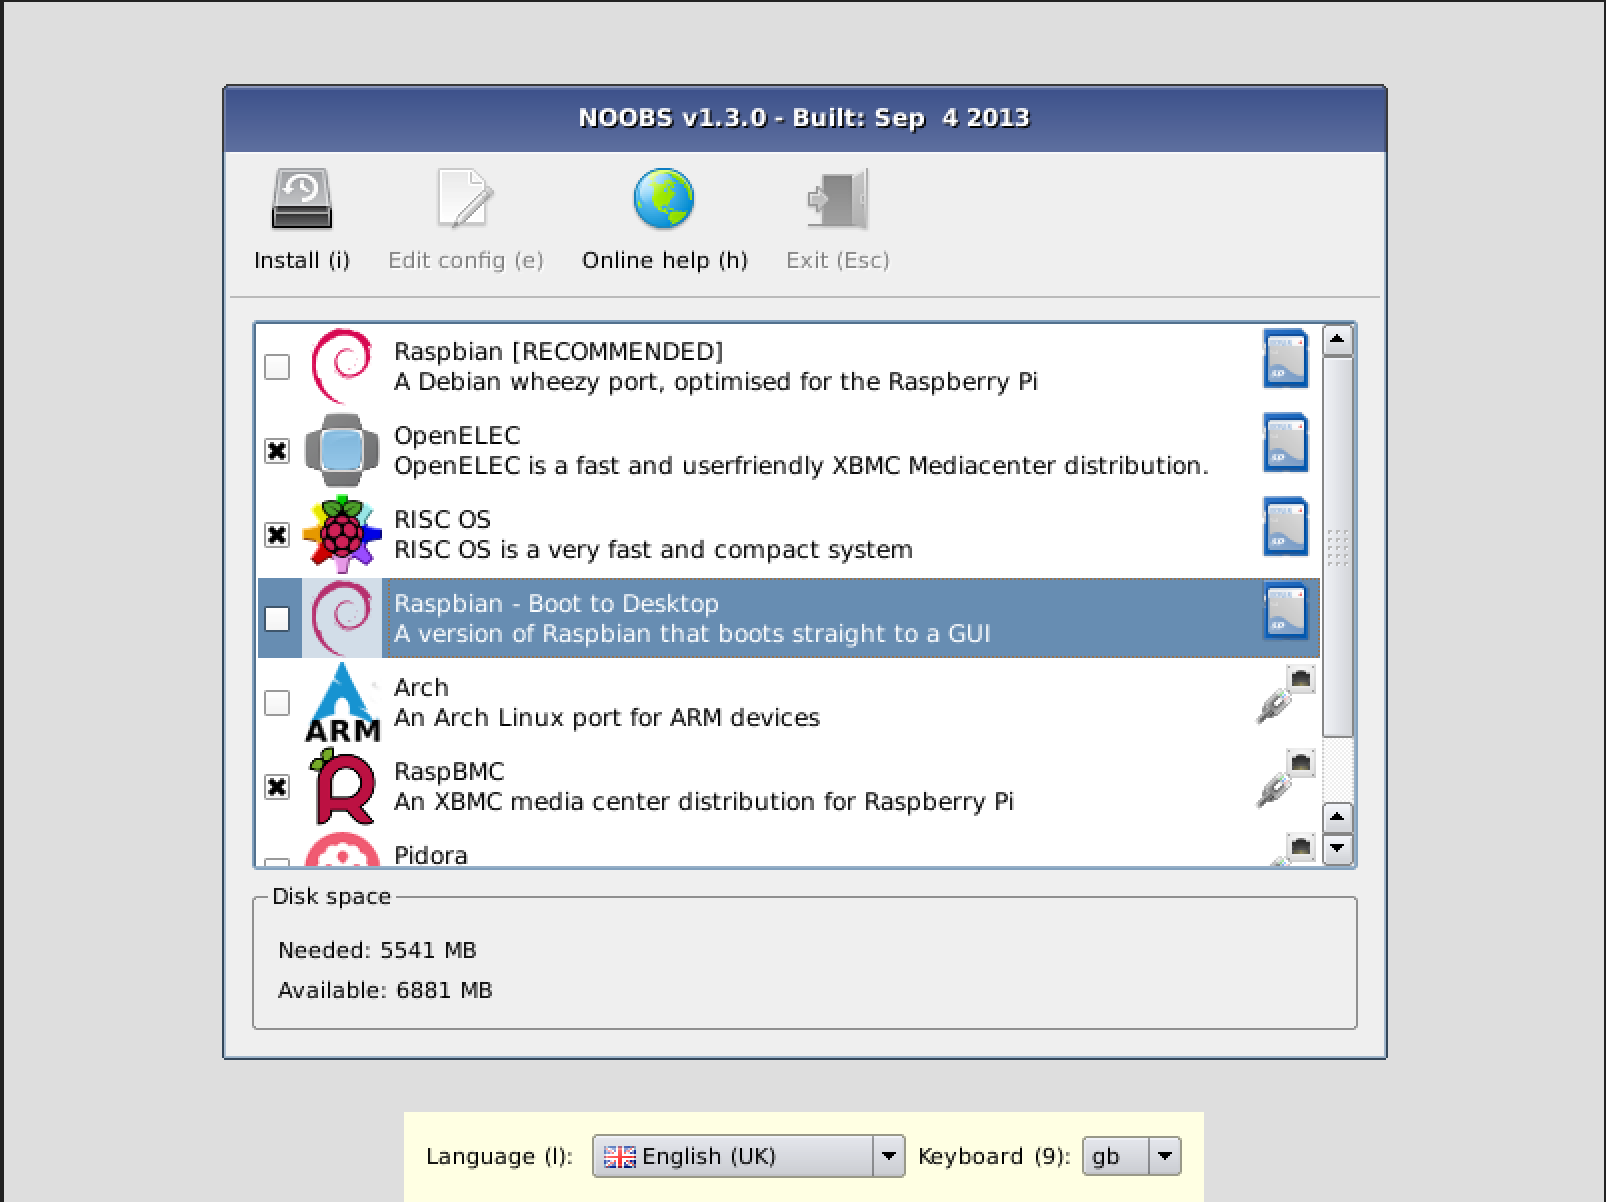
\includegraphics[width=8cm]{guide/5.png}
\end{center}

All'avvio potremo scegliere quale sistema avviare

\end{frame}


\begin{frame}{6) Attendere...}
Attendi che il Raspberry Pi scarichi da internet tutti i sistemi operativi che hai scelto.

\medskip
\begin{center}
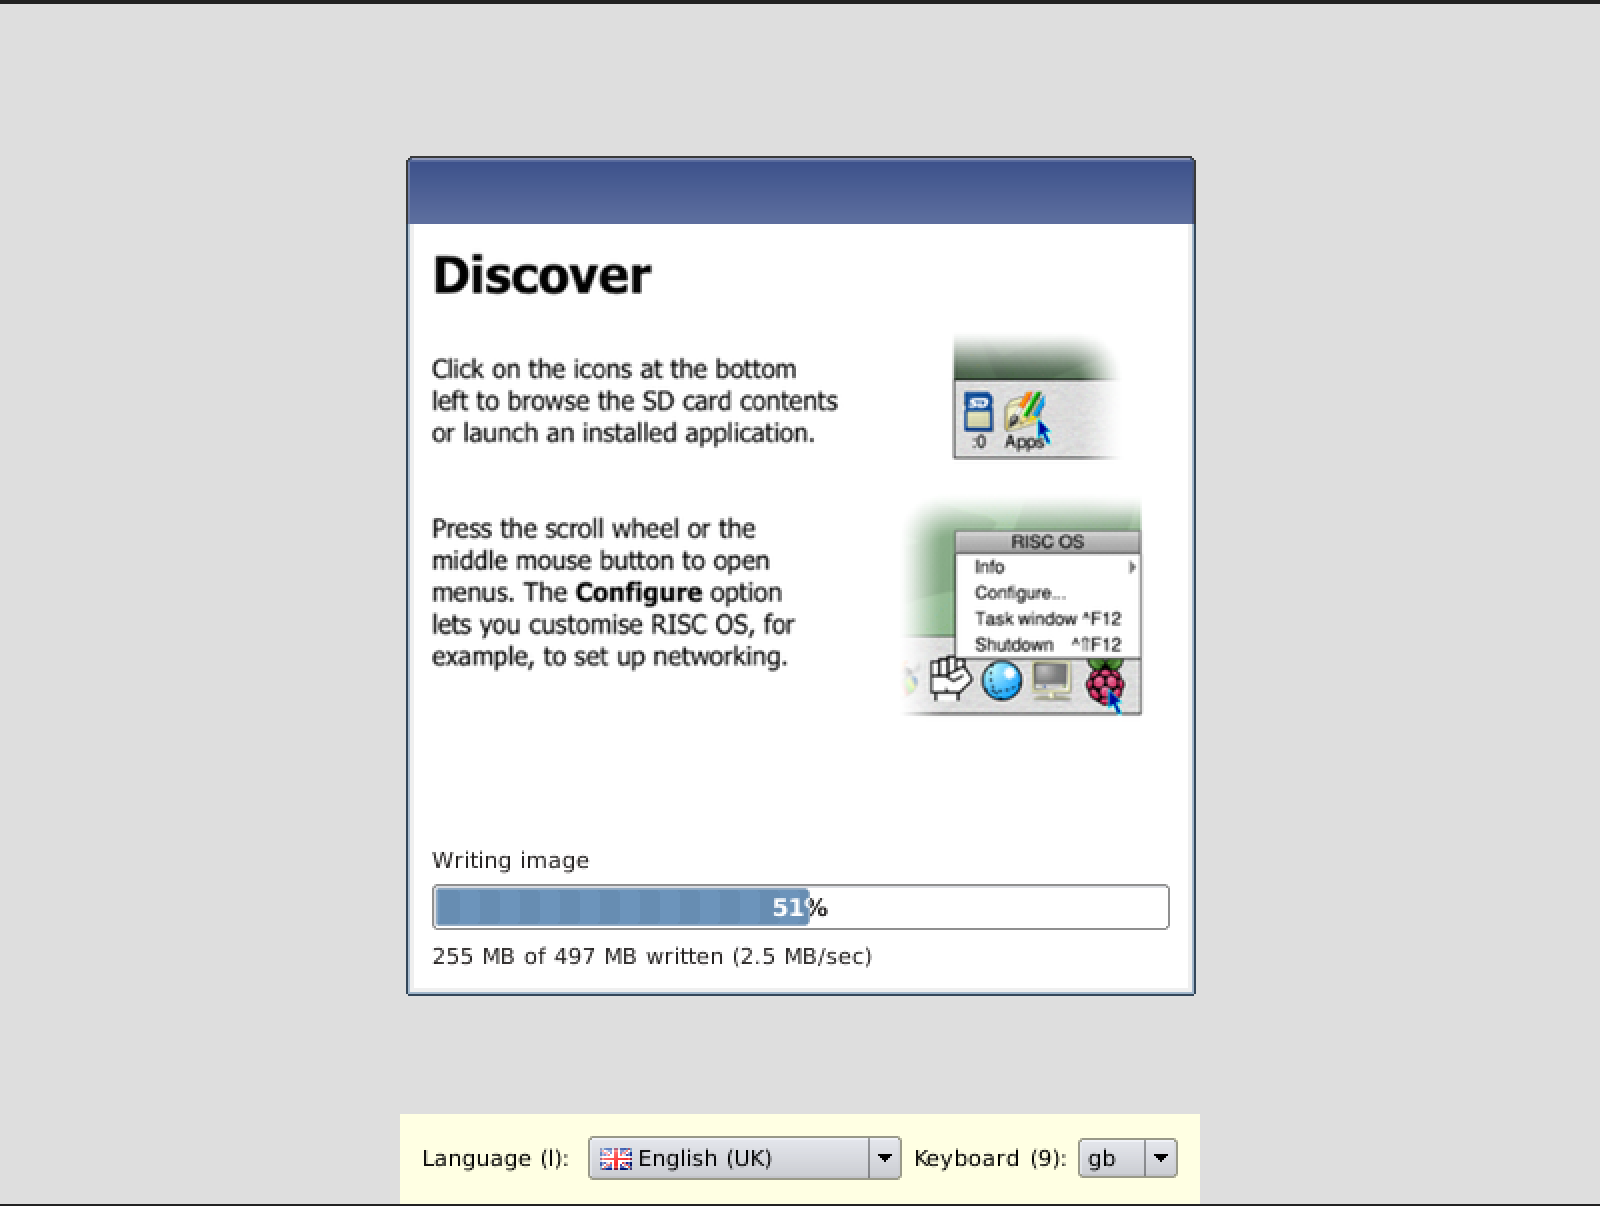
\includegraphics[width=8cm]{guide/6.png}
\end{center}
\end{frame}

%%%%%%%%%%%%%%%%%%%%%%
\section{raspi-config}
\begin{frame}{}
\begin{center}
\begin{Huge}
{\color{green_raspi} \textbf{raspi-config}}
\end{Huge}
\end{center}
\end{frame}

\begin{frame}\frametitle{raspi-config}
\texttt{raspi-config} \`e un tool per \textbf{Raspbian} che ci permette di configurare il nostro Raspberry Pi come meglio vogliamo.
\medskip
\begin{center}
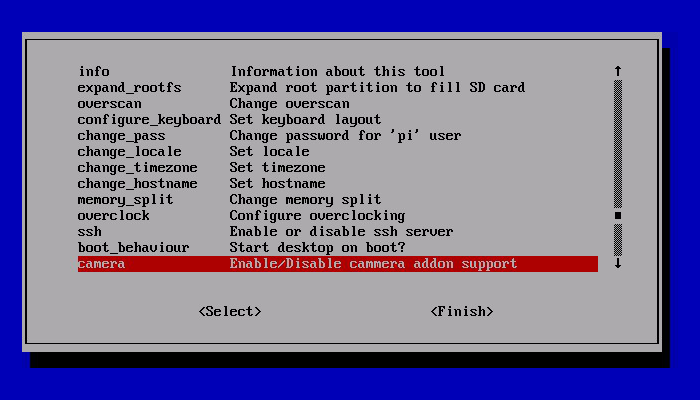
\includegraphics[width=8cm]{raspi-config.png}
\end{center}
\medskip
Vediamo nel dettaglio le varie funzionalit\`a
\end{frame}

\begin{frame}\frametitle{raspi-config}
\begin{description}
  \item[\textbf{Expand Filesystem}] per espandere il filesystem al fine di occupare tutto lo spazio sulla scheda SD (non necessario nel caso di NOOBS).
  \item[\textbf{Change User Password}] per cambiare la password di default (user \textbf{pi} password \textbf{raspberry}).
  \item[\textbf{Boot to Dekstop/Scratch}] per cambiare le opzioni di boot (Desktop, Linea di comando o direttamente su Scratch).
  \item[\textbf{Internationalisation}] per cambiare le impostazioni internazionali (lingua, tastiera, etc.).
\end{description}
\end{frame}

\begin{frame}\frametitle{raspi-config}
\begin{description}
  \item[\textbf{Camera}] per abilitare la Pi-Cam.
  \item[\textbf{Rastrack}] per aggiungere il nostro Raspberry alla mappa di tracciamento globale.
  \item[\textbf{Overclock}] per impostare l'overclock del nostro raspberry (attenzione...).
\end{description}
\end{frame}

\begin{frame}\frametitle{raspi-config (advanced options)}
Abbiamo anche una serie di opzioni avanzate:
\begin{description}
  \item[\textbf{Overscan}] per risolvere problemi di visualizzazione su vecchi monitor (RCA).
  \item[\textbf{Hostname}] per cambiare il nome del Raspberry Pi.
  \item[\textbf{Memory}] per cambiare l'allocazione di RAM fra CPU/GPU.
  \item[\textbf{SSH}] per abilitare il server SSH.
  \item[\textbf{Update}] per aggiornare \texttt{raspi-config}.
\end{description}
\medskip
Abbiamo anche una serie di opzioni avanzate
\end{frame}

%%%%%%%%%%%%%%%%%%%%%%
\section{config.txt}
\begin{frame}{}
\begin{center}
\begin{Huge}
{\color{green_raspi} \textbf{config.txt}}
\end{Huge}
\end{center}
\end{frame}

\begin{frame}\frametitle{config.txt}
Il Raspberry Pi non dispone di un \textbf{BIOS}, tutte le informazioni di boot vengono lette del file \texttt{\textbf{config.txt}}.

\medskip
\pause

Il file si trova nel percorso \texttt{/boot/config.txt}, oppure pu\`o essere editato da un'altro sistema 

\medskip
\pause
\begin{small}
\url{https://www.raspberrypi.org/documentation/configuration/config-txt.md}  
\end{small}
\end{frame}

\begin{frame}[fragile]\frametitle{config.txt}
NOOBS ci auto-configura il file \texttt{config.txt} con le configurazioni ottimali:

\medskip
\pause
\begin{verbatim}
# NOOBS Auto-generated Settings:
hdmi_force_hotplug=1
config_hdmi_boost=4
overscan_left=24
overscan_right=24
overscan_top=16
overscan_bottom=16
disable_overscan=0
start_x=0
gpu_mem=64
\end{verbatim}
\end{frame}

%%%%%%%%%%%%%%%%
\section{Networking}
\begin{frame}{}
\begin{center}
\begin{Huge}
{\color{green_raspi} \textbf{Networking}}
\end{Huge}
\end{center}
\end{frame}

\begin{frame}[fragile]\frametitle{Ethernet}
L'interfaccia Ethernet \`e configurata di default per ottenere un indirizzo IP \textbf{dinamico} tramite \textbf{DHCP}.
\medskip
\`E possibile impostare un indirizzo statico (utile se vogliamo un server domestico) editando il file \texttt{/etc/network/interfaces}.
\begin{verbatim}
iface eth0 inet static
address 192.168.0.123
netmask 255.255.255.0
network 192.168.0.0
broadcast 192.168.0.255
gateway 192.168.0.1
\end{verbatim}
\end{frame}

\begin{frame}[fragile]\frametitle{Ethernet}
Non dimentichiamoci di configurare il DNS nel file \texttt{/etc/resolv.conf}. Aggiungiamo le righe seguenti:
\begin{verbatim}
nameserver 8.8.8.8
nameserver 8.8.4.4
\end{verbatim}

\medskip
Assicuriamoci che la rete funzioni utilizzando i comandi \texttt{ifconfig} e \texttt{ping}.
\end{frame}

\begin{frame}\frametitle{Wireless GUI}
\`E possibile collegarsi alla rete wifi (tramite un dongle usb) utilizzato il tool \textbf{Wifi Config}
\medskip
\begin{center}
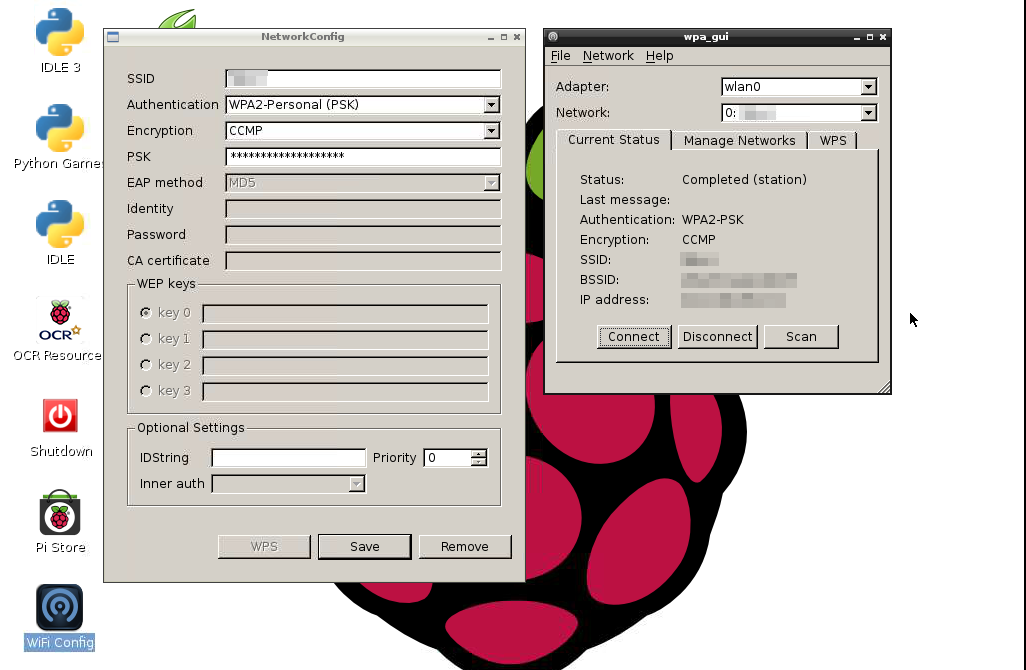
\includegraphics[width=8cm]{wpa-gui.png}
\end{center}
\end{frame}

\begin{frame}[fragile]\frametitle{Wireless CLI}
Nel caso non si disponga di interfaccia grafica \`e possibile indicare una rete a cui connettersi editando il file \texttt{/etc/wpa\_supplicant/wpa\_supplicant.conf}.

\medskip
\begin{verbatim}
network={
    ssid="The_ESSID_aka_Network_name"
    psk="Your_wifi_password"
}
\end{verbatim}
\end{frame}

%%%%%%%%%%%%%%%%
\section{Remote Access}
\begin{frame}{}
\begin{center}
\begin{Huge}
{\color{green_raspi} \textbf{Remote Access}}
\end{Huge}
\end{center}
\end{frame}

\begin{frame}\frametitle{SSH}
Ricordarsi di attivare il \textbf{server SSH} da \texttt{raspi-config}. Cos\`i sar\`a possibile collegarsi da remoto usando il comando:
\medskip
\begin{center}
\texttt{ssh pi \@ [ip\_addr\_raspi]}
\end{center}
Dove \texttt{[ip\_addr\_raspi]} rappresenta l'indirizzo IP del vostro Raspberry (statico o dinamico).
\end{frame}

\begin{frame}\frametitle{SFTP/SCP}
Per trasferire files possiamo usare il comando \textbf{\texttt{SCP}} oppure utilizzare il protocollo \texttt{\textbf{SFTP}}, entrambi si basano su SSH. Possiamo utilizzare un software tipo \textbf{FileZilla} per trasferire files
\medskip
\begin{center}
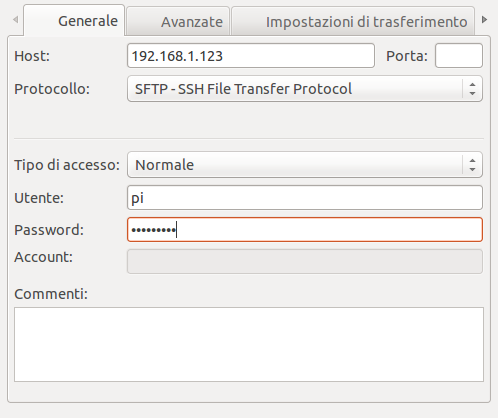
\includegraphics[width=6cm]{filezilla.png}
\end{center}
\end{frame}

\begin{frame}[fragile]\frametitle{VNC}
Per utilizzare il protocollo VNC per aprire una sessione grafica remota sul Raspberry Pi. Configuriamolo sul Raspberry Pi cos\`i:
\medskip
\begin{verbatim}
sudo apt-get install tightvncserver
tightvncserver
vncserver :0 -geometry 1920x1080 -depth 24
\end{verbatim}
Colleghiamoci da un altro computer usando il software \texttt{xtightvncviewer} oppure tramite \texttt{remmina}.
\end{frame}

\begin{frame}\frametitle{DDNS}
    


\end{frame}

%%%%%%%%%%%%%%%%
\section{A simple daemon}
\begin{frame}{}
\begin{center}
\begin{Huge}
{\color{green_raspi} \textbf{A simple daemon}}
\end{Huge}
\end{center}
\end{frame}

\begin{frame}\frametitle{transmission-daemon}
Vedremo adesso come configurare il demone di \texttt{\textbf{transmission}}, un noto client bittorrent per Linux.
\medskip
\begin{center}

\includegraphics[width=5cm]{transmission-icon.png}
\end{center}
\end{frame}

\begin{frame}[fragile]\frametitle{mount}
Per prima cosa dobbiamo assicurarci di avere lo spazio necessario per poter scaricare files. Possiamo utilizzare un hard disk esterno collegandolo ad una delle prese USB del Raspberry Pi.
\medskip
Utilizzando il comando \texttt{sudo fdisk -l} \`e possibile indivuare il nome della periferica e montarla tramite il comando:
\begin{verbatim}
sudo mkdir /mnt/hd
sudo mount /dev/sdaX /mnt/hd
\end{verbatim}
\end{frame}

\begin{frame}\frametitle{mount}
\begin{block}{fstab}
Il mount pu\`o essere anche automatizzato tramite il file \texttt{/etc/fstab} in modo che venga effettuato ad ogni avvio.  
\end{block}

Il file system ottimale \`e \textbf{ext3/4} in quanto \textbf{FAT32} non supporta file di grosse dimensioni, mentre \textbf{NTFS} introduce troppo overhead.
\end{frame}

\begin{frame}[fragile]\frametitle{setup}
Installiamo il demone tramite il comando
\begin{verbatim}
sudo apt-get install transmission-daemon
\end{verbatim}
\medskip
E creiamo due cartelle sulla nostra unit\`a esterna.
\begin{verbatim}
mkdir /mnt/hd/complete
mkdir /mnt/hd/incomplete
\end{verbatim}
\end{frame}

\begin{frame}[fragile]\frametitle{configuration}
Andiamo a configurare il server tramite il file \texttt{settings.json} nella cartella \texttt{/etc/transmission-daemon/}
\medskip
\begin{small}
\begin{description}
  \item[download-dir] La cartella dove vanno i file completi.
  \item[incomplete-dir] La cartella dove vanno i file incompleti.
  \item[incomplete-dir-enabled] True, per abilitare la cartella incomplete.
\end{description}
\end{small}
\end{frame}

\begin{frame}[fragile]\frametitle{RPC}
Configuriamo le impostazioni per l'RPC (Controllo da remoto).
\medskip
\begin{small}
\begin{description}
  \item[rpc-enabled] True per attivare l'RPC.
  \item[rpc-password] Password di accesso.
  \item[rpc-username] Nome utente di accesso.
  \item[rpc-port] Porta su cui \`e in ascolto RPC.
  \item[rpc-whitelist-enabled] False, altrimenti dobbiamo indicare la lista di IP consentiti.
\end{description}
\end{small}
\end{frame}

\begin{frame}[fragile]\frametitle{reload \& restart}
Dobbiamo infine gestire i permessi con questi comandi:
\begin{verbatim}
sudo adduser pi debian-transmission
\end{verbatim}
\medskip
Andiamo nel file \texttt{/etc/init.d/transmission-daemon} e modifichiamo la riga USER= inserendo il proprio nome utente (in questo caso \texttt{pi}).
\medskip
\begin{small}
\begin{verbatim}
sudo chown pi -R /var/lib/transmission-daemon/info/
sudo chown pi /etc/transmission-daemon/settings.json
sudo /etc/init.d/transmission-daemon/reload
sudo /etc/init.d/transmission-daemon/restart
\end{verbatim}
\end{small}
\end{frame}

% \begin{frame}\frametitle{remotes}
% Possiamo adesso gestire il nostro server tramite
% \begin{itemize}
%   \item Interfacce web (\texttt{http://[indirizzo_ip]:9091/})
%   \item Applicazioni quali \textbf{Transmission Remote GUI}
%   \item App mobile quali \textbf{Transmission Remote GUI}
% \end{itemize}
% \end{frame}

% \begin{frame}\frametitle{remotes}
% \begin{center}
% 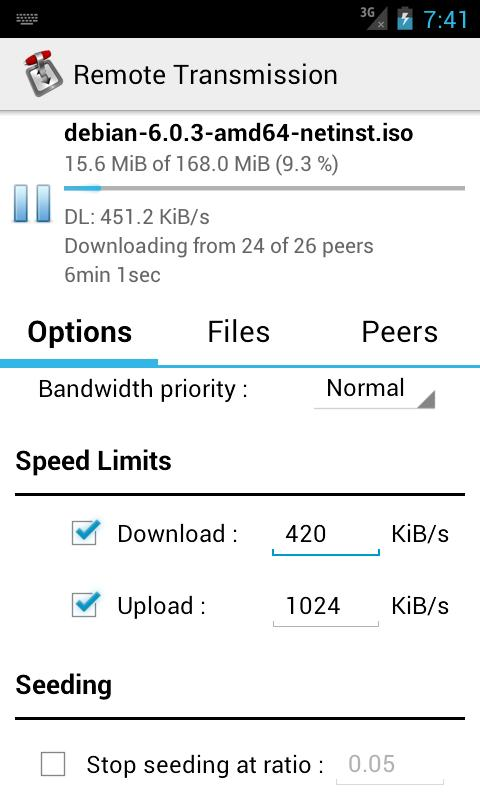
\includegraphics[width=6cm]{remote-android.jpg}
% \end{center}
% \end{frame}

\begin{frame}{}
\begin{center}
\begin{Huge}
{\color{green_raspi} \textbf{Domande...?}}
\end{Huge}

\vspace{1.5cm}
\begin{small}
Slides realizzate da:\\
\textbf{Nicola Corti - corti.nico [at] gmail [dot] com}\\

\bigskip

Slides realizzate con \LaTeX\ Beamer.\\
La seguente presentazione \`e rilasciata sotto licenza\\
\begin{footnotesize}	\textbf{Creative Commons - Attributions, Non Commercial, Share-alike}.
\end{footnotesize}
\\
\medskip

\includegraphics[height=0.5cm]{cc.png}

\end{small}
\end{center}
\end{frame}

\end{document}